\subsection{Routing Table Unit (RTU)}

\noindent {\bf Description:}

RTU is responsible for making the decisions where (to which port or ports of the
Switch) each frame received from any of the ports has to be
forwarded. The decision is made based on the information from:
\begin{itemize}
  \item VLAN table: storing information about the VLAN configuration. Each entry
    contains a mask describing which physical ports belong to the VLAN (each bit
    set to \emph{1} means the port belongs to VLAN), index of VLAN group (FID)
    to which the VLAN belongs to, VLAN-assigned priority and also two additional
    bits, one saying that all frames belonging to the VLAN should be dropped and
    the other saying that every frame belonging to the VLAN should have its
    priority replaced with VLAN priority
  \item Hash table (HTAB): stores dynamic (the result of learning process) and
    static entries describing the presence of MAC addresses on physical ports of
    the Switch (i.e. MAC addresses of the devices connected to each physical
    port of the Switch)
  \item Topology Resolution Unit: responsible for dynamic network topology
    reconfiguration, more detailed description in section \ref{sec:tru}.
\end{itemize}

The Hash Table contains a set of MAC entries of the structure presented in the
table:\\

\noindent
\resizebox{\textwidth}{!}{
\begin{tabular}{|>{\centering\arraybackslash}p{1cm}|c|c|p{3cm}|p{8cm}|}
  \hline
  {\bf word no.} & {\bf offset} & {\bf length} & {\bf name} & {\bf description}\\
  \hline \hline
  \multirow{9}{*}{0} & 0 & 1 & \texttt{valid} & if 1, the entry contains valid data\\
  \cline{2-5}
  & 1 & 1 & \multicolumn{2}{l|}{\emph{reserved}}\\
  \cline{2-5}
  & 2 & 1 & \texttt{is\_bpdu} & if 1, accept frame even if the port is disabled in RTU
  configuration\\
  \cline{2-5}
  & 3 & 1 & \texttt{go\_to\_cam} & obsolete, will be removed or replaced\\
  \cline{2-5}
  & 4 & 8 & \texttt{fid} & Filtering Database ID which was used to generate the address
  (hash) of the entry\\
  \cline{2-5}
  & 12 & 4 & \multicolumn{2}{l|}{\emph{reserved}}\\
  \cline{2-5}
  & 16 & 16 & \texttt{mac[47:32]} & MAC address (high part)\\
  \hline \hline
  1 & 0 & 32 & \texttt{mac[31:0]} & MAC address (low part)\\
  \hline \hline
  \multirow{18}{*}{2} & 0 & 16 & \texttt{cam\_addr} & obsolete, will be removed or replaced\\
  \cline{2-5}
  & 16 & 1 & \texttt{has\_prio\_src} & validates prio\_src and prio\_override\_src
  fields\\
  \cline{2-5}
  & 17 & 3 & \texttt{prio\_src} & priority of the frame having source MAC matching with
  MAC of this entry\\
  \cline{2-5}
  & 20 & 1 & \texttt{prio\_ \linebreak override\_src} & override frame's priority with
  \emph{prio\_src} when its SMAC matches MAC of this entry\\
  \cline{2-5}
  & 21 & 1 & \texttt{drop\_when\_src} & drop frame when its SMAC matches MAC of this
  entry\\
  \cline{2-5}
  & 22 & 1 & \texttt{drop\_when\_ \linebreak unmatched\_ \linebreak src\_ports} & drop the frame when it comes
  from source port which does not belong to port\_mask\_src\\
  \cline{2-5}
  & 23 & 1 & \texttt{has\_prio\_dst} & validates prio\_dst and prio\_override\_dst\\
  \cline{2-5}
  & 24 & 3 & \texttt{prio\_dst} & priority of the frame having DMAC matching with MAC 
  of this entry\\
  \cline{2-5}
  & 27 & 1 & \texttt{prio\_ \linebreak override\_dst} & override frame's priority with
  \emph{prio\_dst} when its DMAC matches MAC of this entry\\
  \cline{2-5}
  & 28 & 1 & \texttt{drop\_when\_dst} & drop frame if its DMAC matches MAC of this
  entry\\
  \hline \hline
  \multirow{10}{*}{3} & 0 & 16 & \texttt{port\_mask\_ \linebreak src[15:0]} &
  low part of the port mask for SMAC, bit set
  to 1 indicates that frame with SMAC matching MAC of this entry can be
  forwarded from that port/ports. Ports having their bits set to 0 shall drop
  the frame\\
  \cline{2-5}
  & 16 & 16 & \texttt{port\_mask\_ \linebreak dst[15:0]} & low part of the port mask for DMAC, bit set
  to 1 indicates to which physical ports the frame with DMAC matching MAC of
  this entry shall be forwarded\\
  \hline \hline
  \multirow{4}{*}{4} & 0 & 16 & \texttt{port\_mask\_ \linebreak src[31:16]} &
  high part of the port mask for SMAC\\
  \cline{2-5}
  & 16 & 16 & \texttt{port\_mask\_ \linebreak dst[31:16]} & high part of the port mask for DMAC\\
  \hline
\end{tabular}
}

\vspace{12pt}
HTAB is organized in buckets. Each bucket stores five words of MAC entry
described in the table above. The bucket is addressed with the hash value
calculated from the FID and MAC address of the MAC entry it stores. This hash is
a CRC generated using one of the supported polynomials (\emph{POLY\_VAL} of GCR
Wishbone register). Since different MACs and FIDs can result in the same hash
value, each of the hash is associated with four buckets. If it turns out that
first bucket already stores a valid MAC entry, next one is checked. A new MAC
entry is then written to first free (not already used) bucket.

HTAB is written by the switch software and can contain both static entries
required by the configuration of the Switch and dynamic entries resulting from
learning process implemented in software. Write-only access to HTAB is provided
through MFIFO Wishbone registers (\emph{MFIFO\_R0}, \emph{MFIFO\_R1} and
\emph{MFIFO\_CSR}). The address of this memory has the structure presented in
figure \ref{fig:rtu:htab_adr}.

\begin{figure}[ht]
  \begin{center}
    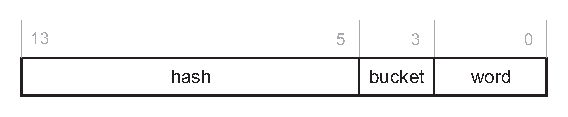
\includegraphics[width=.7\textwidth]{switch/rtu_mfifo_adr.ps}
  \end{center}
  \caption{Structure of HTAB address}
  \label{fig:rtu:htab_adr}
\end{figure}

To write a new MAC entry to HTAB first you have to write an address where the
first word of MAC entry will be written (least significant three bits -
\emph{word} - of the HTAB address equal 0) and then continue writing word by
word a complete entry:

\begin{tabular}{c|l}
  {\bf register} & {\bf value}\\
  \hline
  \texttt{MFIFO\_R0} & \emph{0x01}\\
  \texttt{MFIFO\_R1} & $<$HTAB address$>$\\
  \texttt{MFIFO\_R0} & \emph{0x00}\\
  \texttt{MFIFO\_R1} & $<$word 0$>$\\
  \texttt{MFIFO\_R1} & $<$word 1$>$\\
  \texttt{MFIFO\_R1} & $<$word 2$>$\\
  \texttt{MFIFO\_R1} & $<$word 3$>$\\
  \texttt{MFIFO\_R1} & $<$word 4$>$\\
\end{tabular}\\

The dynamic entries in HTAB should be created by learning mechanism based on the
information got from HDL through UFIFO (when learning on a port is enabled). RTU
module is capable of generating an interrupt when UFIFO is not empty i.e. it
stores at least one learning request. The UFIFO provides basic information
about the unrecognized frame: source MAC, destination MAC, optionally VLAN Id
and priority.\\

The RTU contains also the memory called ARAM which stores an aging bitmap. Each
bit corresponds to one MAC entry in HTAB and, when set to \emph{1}, indicates
that the MAC entry has been matched with the source MAC of the forwarded frame. The
memory is addressed in a similar way as HTAB, but since here each bit
corresponds to one MAC entry and each word is 32-bits long, the word in ARAM
is addressed with address from figure \ref{fig:rtu:htab_adr} shifted 8 bits to
the right (i.e. hash[8..3]). Three least significant bits of hash value
concatenated with the bucket number are used to find an appropriate bit in the word
read from the ARAM.\\

Besides the basic functionality described above, RTU has two main extensions:
\begin{itemize}
  \item {\bf port mirroring}: allows the ingress or egress traffic from selected
    port to be retransmitted on one or multiple other ports configured with
    appropriate mask
  \item {\bf Fast Match mechanism}: provides quick (23 clock cycles in worst case)
    routing response for selected types of frames
\end{itemize}

Fast Match can generate routing responses for (if appropriate bits are set in
\emph{RX\_CTR} control register):
\begin{itemize}
  \item broadcast frames: DMAC is FF:FF:FF:FF:FF:FF
  \item PTP frames: DMAC is 01:1B:19:00:00:00
  \item Link-Limited frames: DMAC in range from 01:80:C2:00:00:00 to
    01:80:C2:00:00:0F
  \item High Priority frames: which have priority included in the
    \emph{PRIO\_MASK} of \emph{RX\_CTR} register
  \item Any frame that has its DMAC in configured range of MAC addresses or DMAC
    equal to single configured MAC
\end{itemize}

\noindent{\bf Wishbone interface:} section \ref{subsec:wbgen:rtu}\\
